\chapter{Activity Diagrams}

\section{Description}
The activity diagrams show the potential paths of actions a user may take with the system. For the Resident actor (Figure \ref{fig:residentdiagram}), upon turning on a system, the user may register or remove devices. The system will be then available and a user may receive a response when the doorbell is pressed. From any of these actions a user may take, they may also power the system off. For the Visitor actor (Figure \ref{fig:visitordiagram}), when the system is on, the user will be able to activate the doorbell by a button and have one of the connected devices respond to the Resident actor.

\begin{figure}[h]
  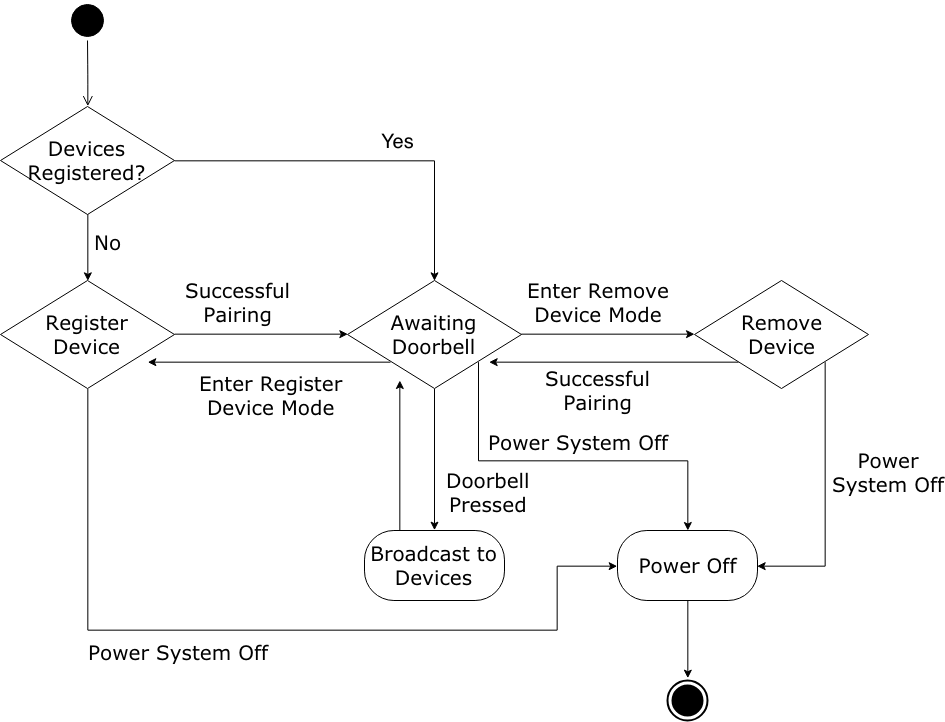
\includegraphics[width=0.8\textwidth]{ResidentActivityDiagram.png}
  \centering
  \caption{Resident Activity Diagram}
  \label{fig:residentdiagram}
\end{figure}

\begin{figure}[h]
  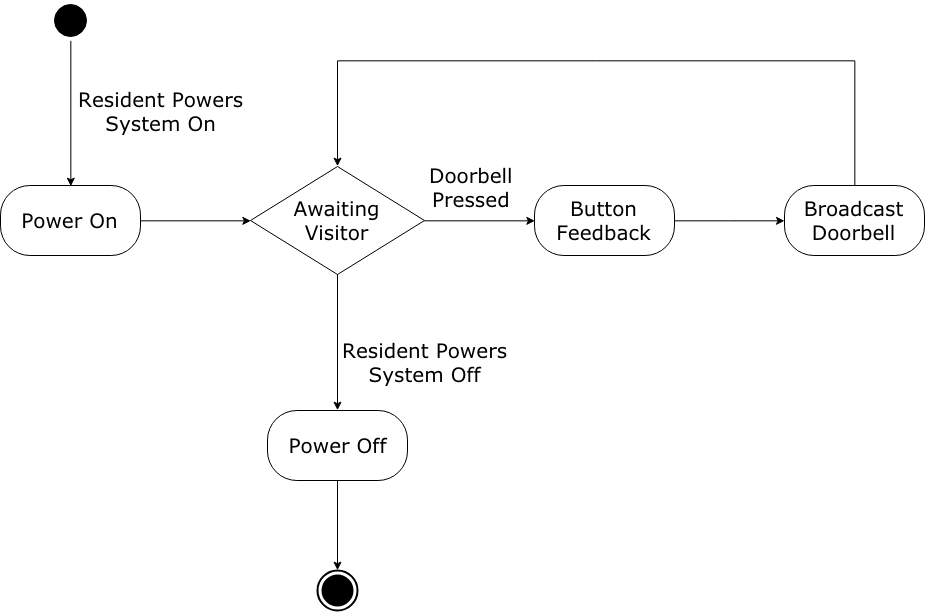
\includegraphics[width=0.8\textwidth]{VisitorActivityDiagram.png}
  \centering
  \caption{Visitor Activity Diagram}
  \label{fig:visitordiagram}
\end{figure}